%%%%%%%%%%%%%%%%%%%%%%%%%%%%%%%%%%%%%%%%%%%%%%%%%%%%%%%%%%%%%%%%%%%%%%%%%%%%%%%%
%
%   Semester project, fall term 2014
%   Author: Jakob Ehrl, born 01/24/91
%   Study program: Computer science, MA 1
%   
%   Professor Dr. Francesco Mondada
%   Assistant: Dr. Stefan Witwicki
%
%%%%%%%%%%%%%%%%%%%%%%%%%%%%%%%%%%%%%%%%%%%%%%%%%%%%%%%%%%%%%%%%%%%%%%%%%%%%%%%%%

\chapter{Modules}

All the robot's main functions: actuations, processing and sensing, were performed by different modules. The reason for this separation was to have microcontrollers dedicated for one purpose, thus optimizing the calculation time and efficiency of the robot. In our robot, Four main modules were working together, and each of them had specific roles.

\section{Sensors Module}
The sensors Module is an arduino micro that is connected to the following
\begin{itemize}
\item 5 Infrared sensors, for obstacle detection.
\item 4 Ultrasound sensors, for bottle detection.
\item One DC brush motor driver, for the control of the frontal brush.
\end{itemize}

The task of the Arduino is to constantly receive data from the ranging devices, as well as the current measurements from the DC motor driver, transmit its data to the central processing module, and if commanded to do so, control the driver which is connected to the frontal brush motor. 

\subsection{Sensor Choices and Strategy}
During the first weeks of the semester, different sensors were purchased, and tests were performed on them, in order to have a better choice for the selection of the sensors that would be used on the robot. 


\subsubsection{The Infrared Sensor}
The Infrared sensor that was available from the virtual marked was a GP2Y0A21YK, a sensor from Sharp. 

\begin{figure}[H]
  \centering
  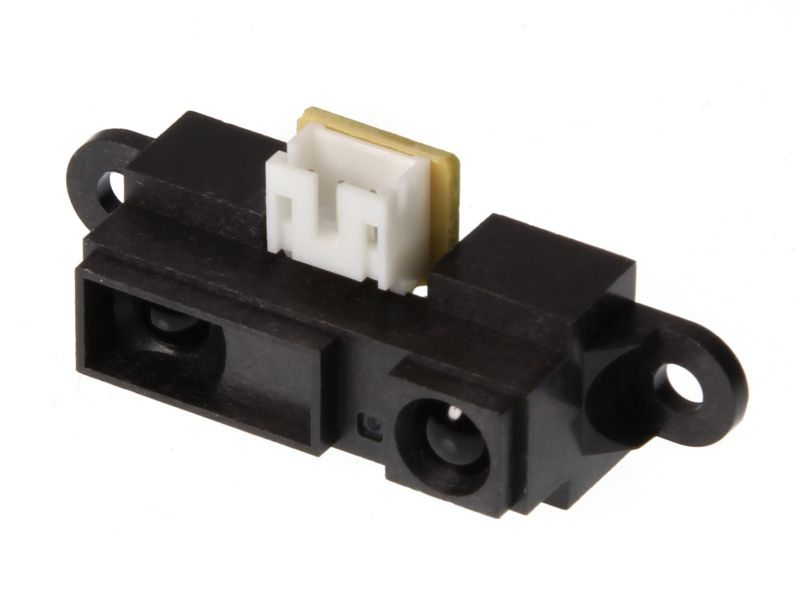
\includegraphics[width=0.3\textwidth]{IR.jpg}
  \caption{GP2Y0A21 Infrared sensor.}
\label{fig:IR}
\end{figure}

The sensor had a range up to 80 cm, which was quite far, however it had some problems detecting transparent bottles, as the IR wave would go through the bottle. Therefore, the sensor was used in detecting obstacles and solid opaque objects, as a collision avoidance strategy. In the robot, 5 of those sensors were used, two in the front, one on each side, and one on the rear, for controlling collisions while going backwards.

For measuring the distance effectively, as the relation between the voltage output of the sensor and the distance was not linear, a linear regression method was used with the measured values in the datasheet of the sensor.

\subsubsection{The Ultrasonic Sensor}

The HC-SR04 is a ultrasonic sensor, that functions with two signals: Echo and Trig. For simplicity, it was tested to combine these two lines into one, with a resistance in between, and changing the state of the pin on the arduino everytime we would measure the signal. However, tests proved that the sensor worked less well than with two pins in this configuration, so two pins were used instead. The range was up to 4 meters, however, as this range was useless, the range was decreased to 1.3 meters. The decrease in range also allowed the signal to be faster, since the arduino is waiting for a pulse input when reading the sensor value, and at closer range the pulse comes back faster. A timeout was used to enforce the range limitations. 

\begin{figure}[H]
  \centering
  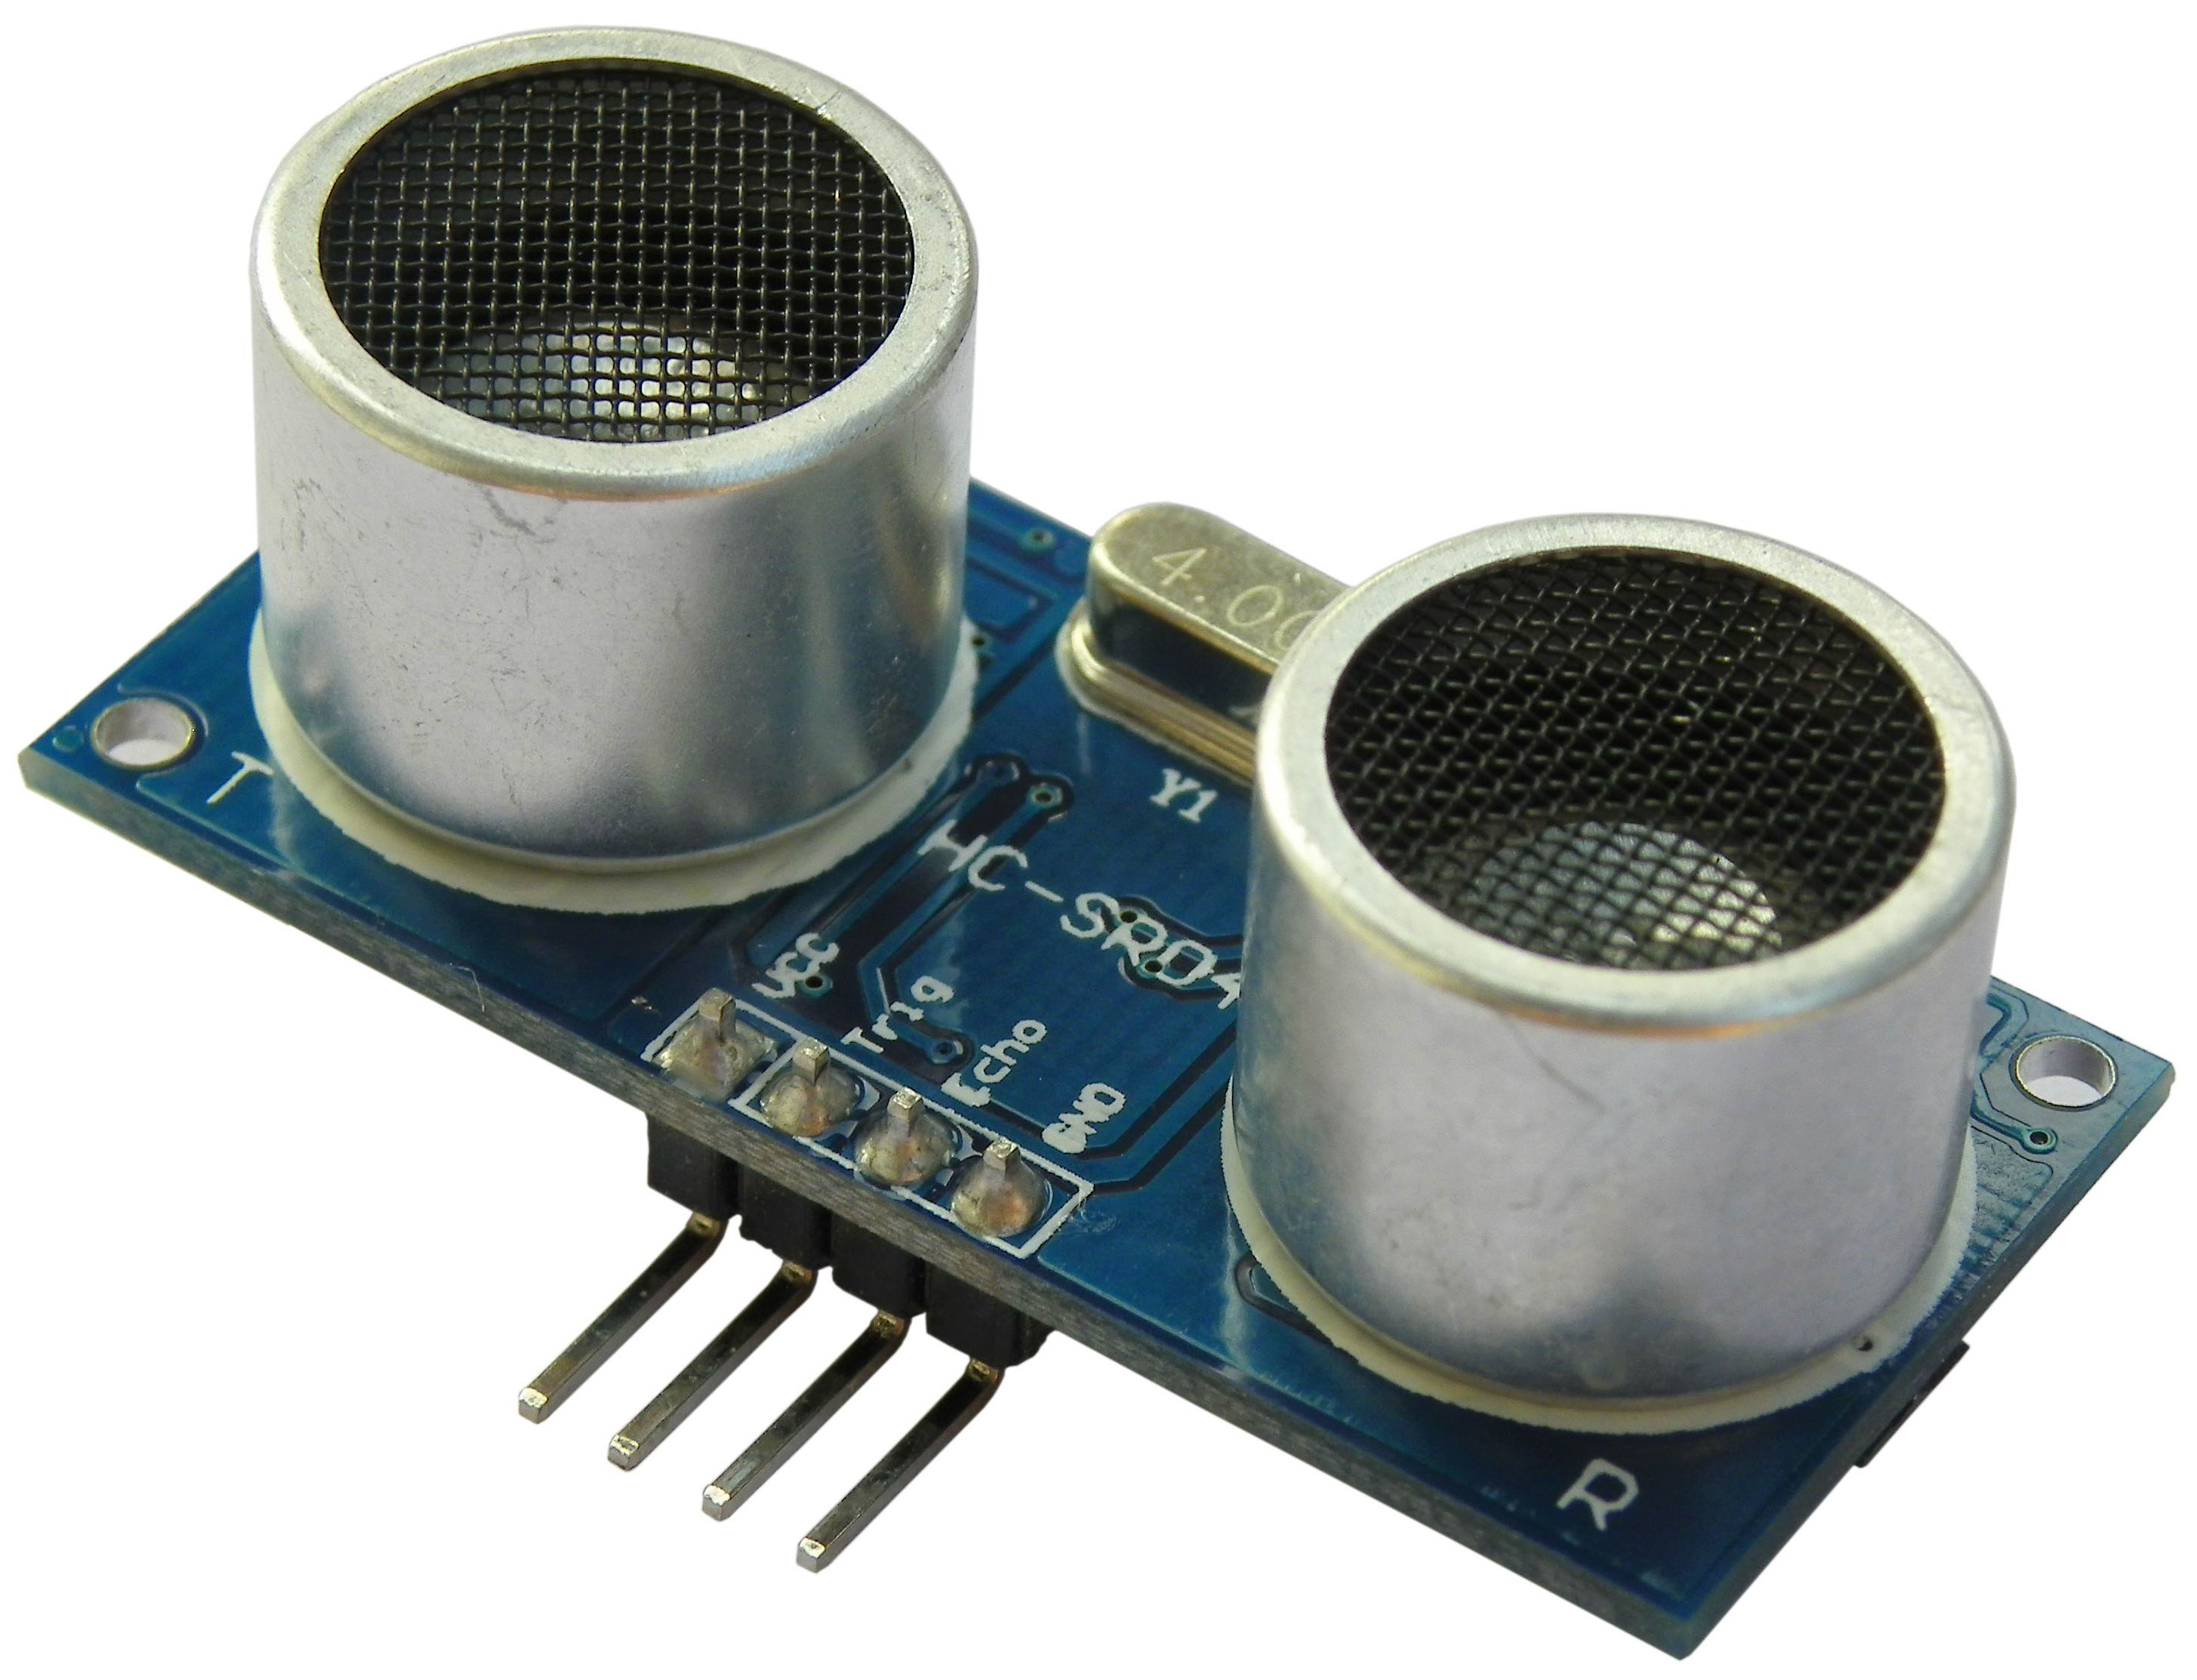
\includegraphics[width=0.3\textwidth]{US.jpg}
  \caption{HC-SR0 Ultrasonic sensor.}
\label{fig:US}
\end{figure}

All in all, the sensor worked quite well with complex shaped objects, but on a flat surface that is not perpendicular to the sensor, the sound wave is bounced on the side, so it is not working.

Ultrasonic sensors were supposed to be close to the ground to measure the position of possible bottles, and could help maneuver the robot in the right path before seeing them with it's camera. However, problems occured during the implementation of the four sensors on the robot, and they were finally not used by the robot, and replaced with infrared sensors.

\subsubsection{The Disposal of the Proximity Sensors}

The idea behind the disposal of the sensors on the robot was to easily allow it to distinguish among bottles and obstacles (that could be either bricks or walls). In order to do so both ultrasonic and infrared sensors were supposed to work together in order to distinguish whether the sensed object was an obstacle or a bottle, by comparing two height of sensors that pointed in the same direction.

To avoid any possible ambiguity we arranged the disposal of the IR in a way that every time they detected something it had to be an obstacle.
This was possible by exploiting the previous knowledge that there is always a gap between the highest point of a bottle on the terrain and an obstacle whether it was a brick or a wall.
Therefore we placed the IR on supports and at an height of 25 cm that is comprised in the range between a standing bottle (max 22 cm) and a brick (28 cm).
Four Infrared sensors were used in the frontal part of the robot.

During the tests, it was shown that two additionnal IR sensors were necessary at the rear part of the robot in order to avoid properly the obstacles.

One more Infrared proximity sensor is present in the back of the robot.
However, this is the only one, of the 5 IR, not respecting the position in the gap described by a standing bottle and a brick.

This has been considered unnecessary since during the performance the robot has to move mainly forward and the only time where it has to move backward is avoid obstacles. As a result it would be useless to distinguish an obstacle from a bottle in such a situation since otherwise the robot would have to perform a difficult maneuver turning of 180°.
This explains also why we decided to put 6 Infrared sensors pointing forward, and only one pointing back: most of the time the robot has to move forward so it doesn’t care about detecting obstacles behind it.
Thus IR in our case have been used solely for pure obstacle avoidance.

On the other hand the ultrasonic sensors had a role (as well as the camera) in bottle detection.
Two of them were placed at the extremities of the elevator allowing to detect the bottles that would partially fall out of the elevator's boundaries. In this way the trajectory of the robot can be corrected, centering the bottle and increasing the possibilities of grasping it in the desired way.

If the bottle is perfectly aligned with the robot since the beginning, no maneuvers would be required .
One of the reason that brought us to use the ultrasonic sensors for this scope and the IR for pure obstacle avoidance was that the Ultrasonic sensors have a way bigger range of detection, allowing to correct the trajectory in time to aim to the bottle in the best position possible.
The other reason was purely due to the constraints given from our choice of the electronic to use.

To sum up, comparing infrared and ultrasonic sensor it can be said that the infrared sensor is easier to use, but presents drawbacks as the influence of the ambient light and the albedo of the reflecting object, while the ultrasonic sensor is not affected by these situations. In addition, the ultrasonic sensor can measure longer distances, until
several meters if the object is well-oriented (inclination of the object to detect smaller than 45° even if the further the object the smaller this angle of tolerance), when the infrared sensor can not detect something beyond 80cm and is way less precise.
Moreover, the infrared sensor is not reliable in the detection of bottles, due to the plastic transparent part, and receive often inconsistent data in return as the light is partially reflected.

\begin{figure}[H]
  \centering
  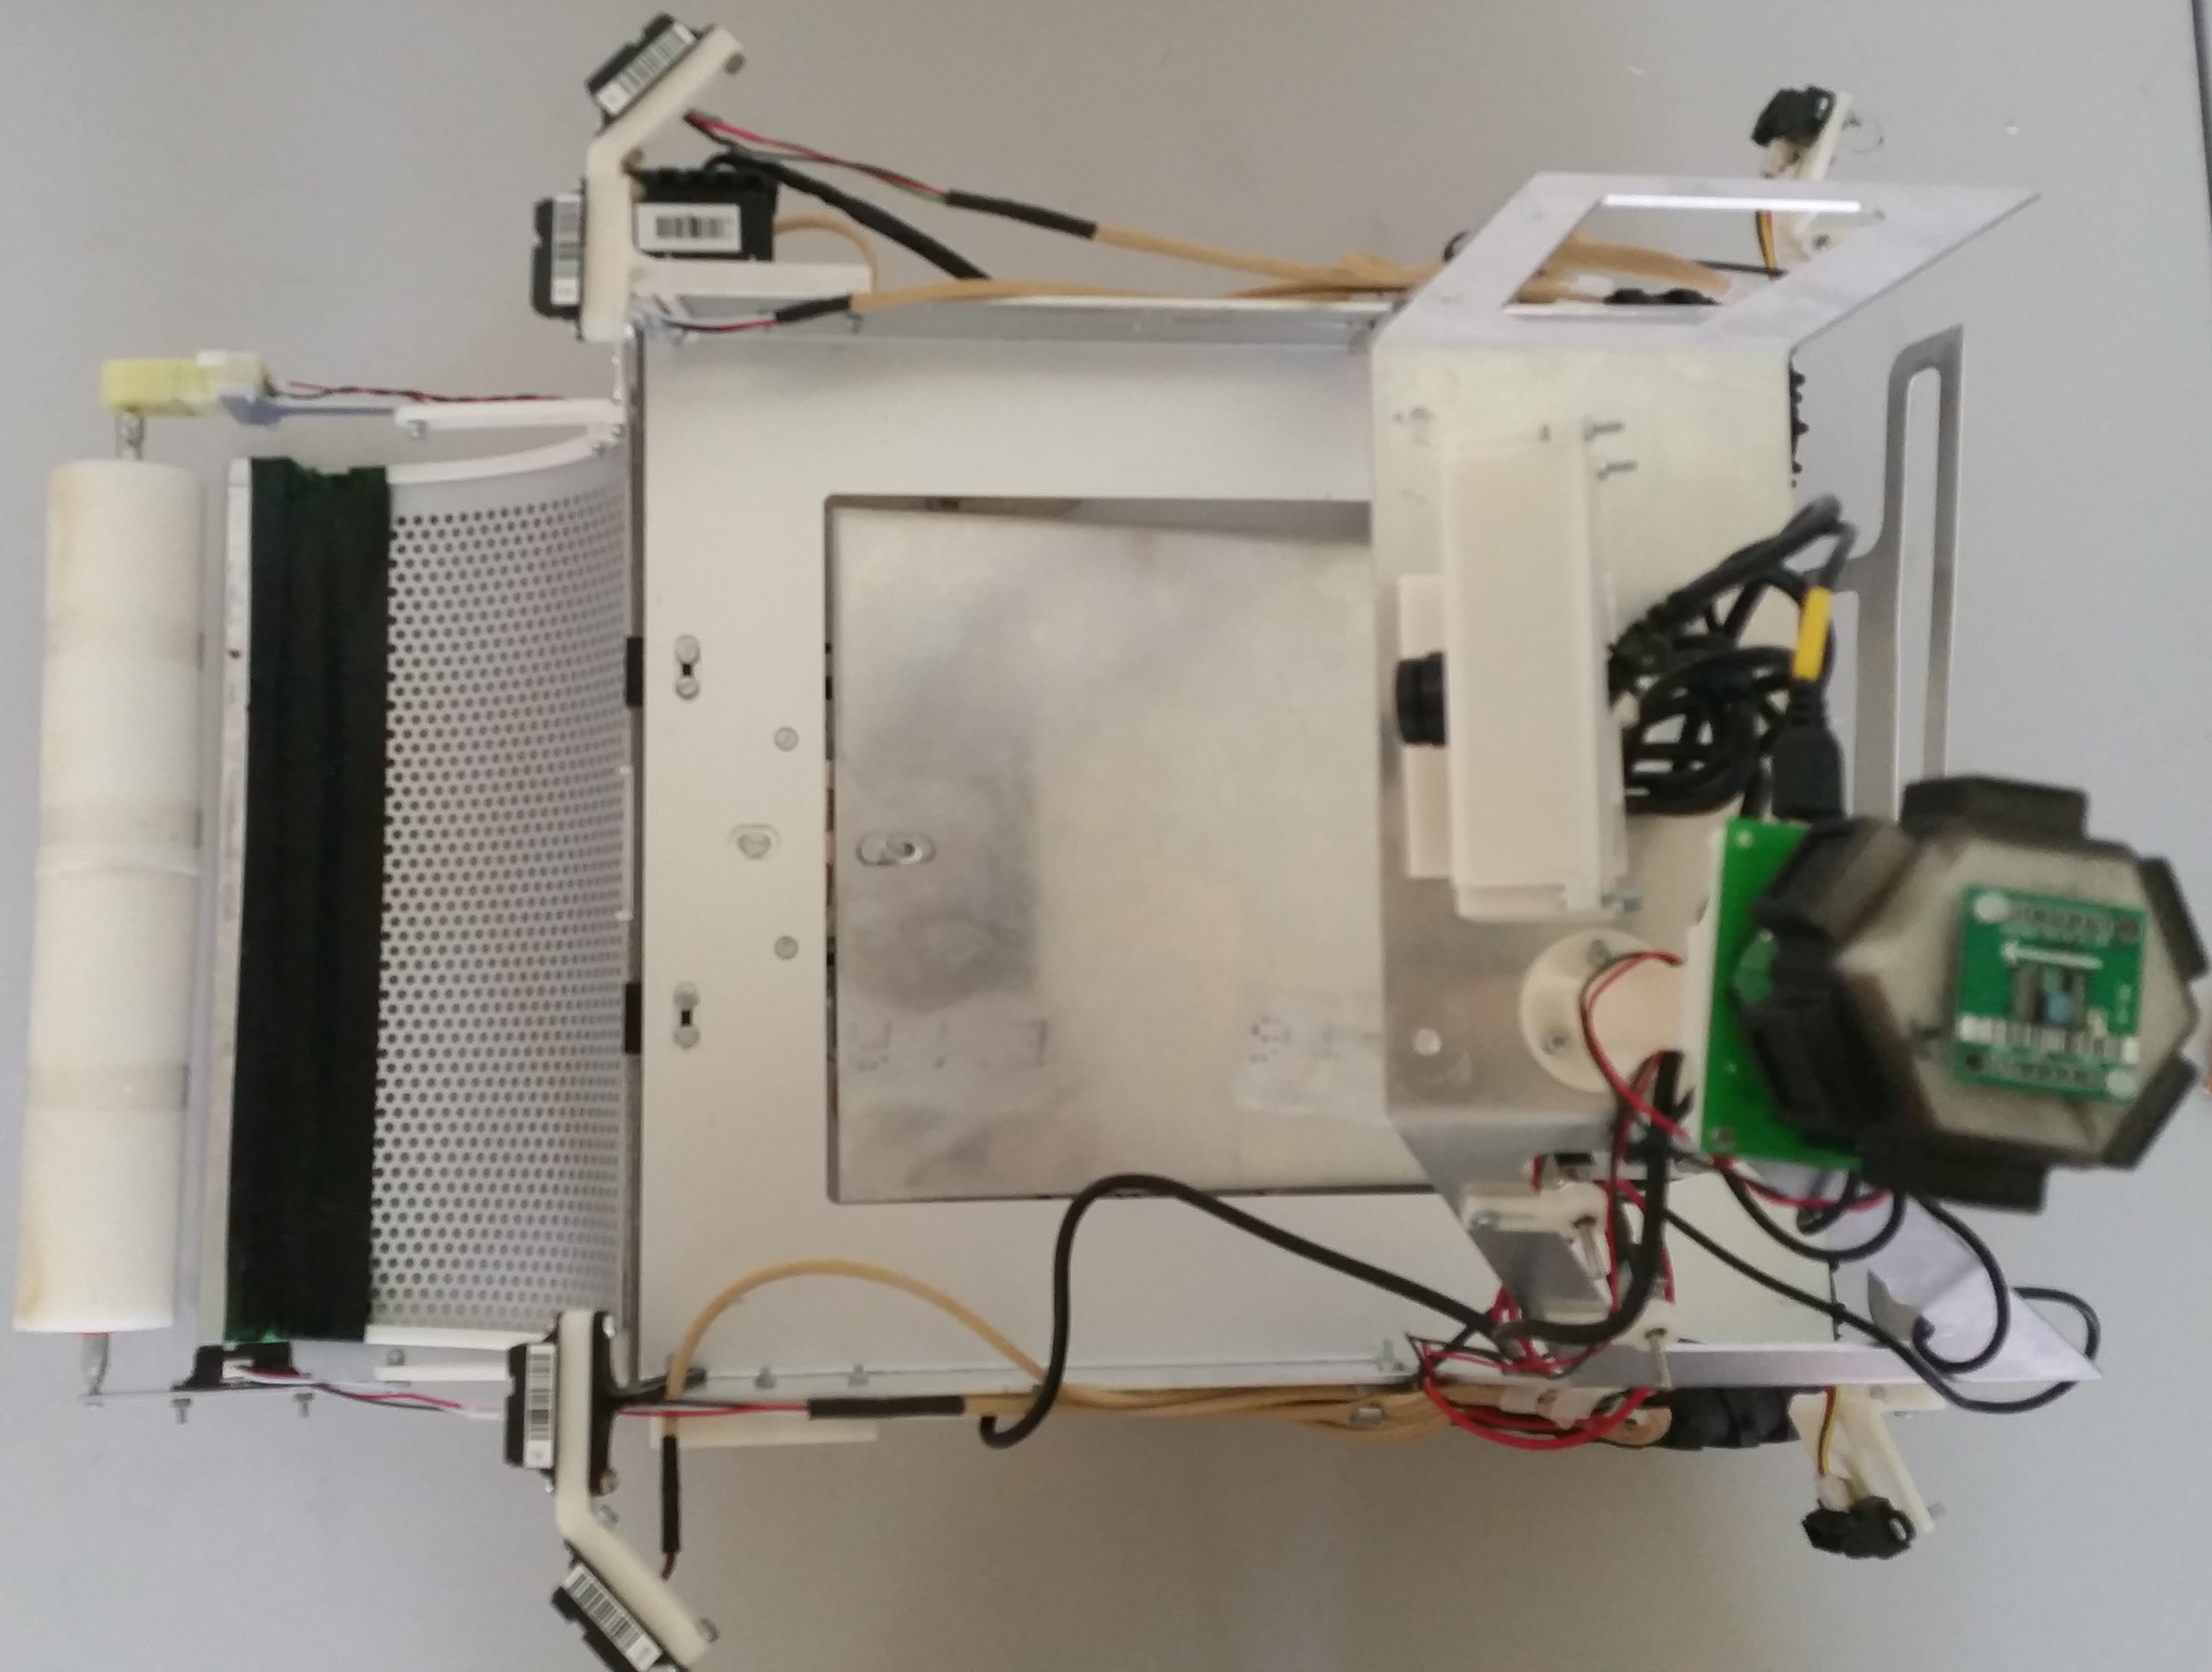
\includegraphics[width=0.4\textwidth]{robottop.jpg}
  \caption{The top view of the robot.}
\label{fig:robottop}
\end{figure}

Finally, The disposition of the sensors was changed before the competition. As in \ref{fig:robottop}, the ultrasonic sensors were removed, and 8 infrared sensors were used instead. The bottle detection worked with the camera, so the ultrasonic sensors became useless.

\subsection{Brush Motor and driver}

For the frontal brush, we needed to have a light but quite powerful motor, which could help pulling the bottles towards the inside of the robot's 'shovel'. We decided to order a $180:1, 2.2 kg\cdot cm$ motor at $4.5 volts$ bought in pololu (see Figure \ref{fig:brushmotor}).

\begin{figure}[H]
  \centering
  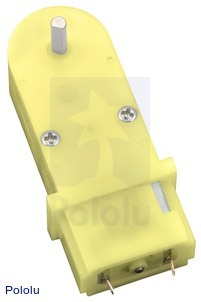
\includegraphics[width=0.2\textwidth]{brushmotor.jpg}
  \caption{A VNH5019 Motor driver Carrier.}
\label{fig:brushmotor}
\end{figure}

Agter testing this motor with bottles, we agreed on keeping it, as it was quite lightweight at a little less than 20 grams, and it worked quite well on picking up bottles. 

In order to anticipate a blocked bottle, or helping counting the number of bottles taken, a motor driver with current sense was bought, that would control the plastic motor. As the choice of motor drivers with current sense ability was quite limited, and adequate for our motor, we had no other choice than to take one that went out of the specifications recommended for the motor.

\begin{figure}[H]
  \centering
  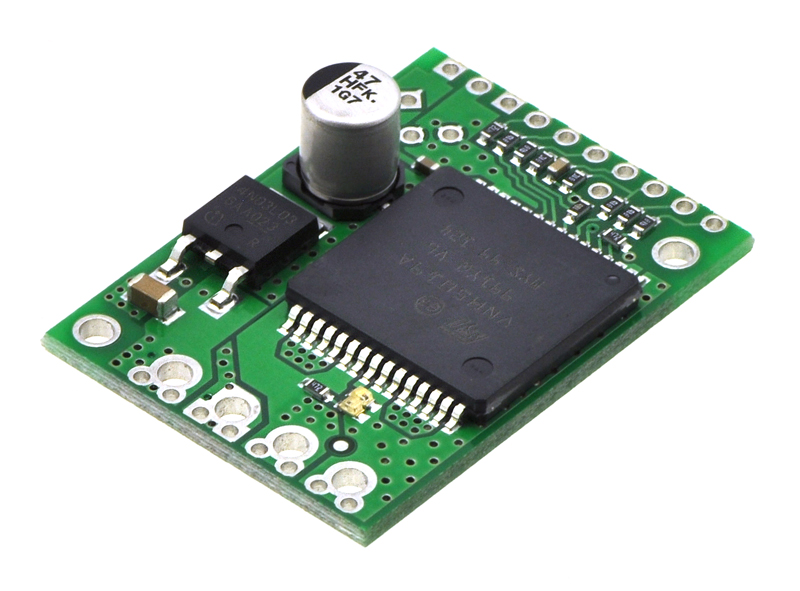
\includegraphics[width=0.3\textwidth]{driver.jpg}
  \caption{A VNH5019 Motor driver Carrier.}
\label{fig:driver}
\end{figure}

With the VNH5019 (See Figure \ref{fig:driver} above), the voltage supply was minimum $5.5 volts$, so we decided to supply the motor directly from the battery. After some research and testing, it was found that the motor works well under those conditions, if the PWM us not at the maximum. For this, the maximum average voltage supplied by the driver in PWM was kept under $4.5 V$ as recommended by the constructor.

The VNH5019 Driver for the plastic gearmotor had a current sense ability that was implemented at 140mV/A. With the arduino micro, an analog input was used to measure this voltage. At 1023 increments for a nominal voltage of 5 Volts, we can measure with a precision of $4.9 mV$ per increment. This meant that we could measure with a precision of $140/4.9 = 28 increments / Amp$, so a resolution of 35mA. As our motor had a stall current of 800mA, we judged the resolution enough for counting the bottles picked up. After some tests, we could confirm this choice as the current was clearly increasing when the bottles were being taken.

When testing this function in practice, it occured to us that the sensing data was only noise. All the wires were close to the motors, and the electromagnetic field induced false measurements. The increments were also too small to be sensed accurately, so instead we used an infrared sensor to detect the presence of bottles.

\subsection{Shovel actuaction}

For the rotating movement of the frontal shovel, the best solution was to find a servomotor powerful enough for rotating the whole shovel upwards. With a high torque of 1.5Nm, and a relatively low price, the actuator of choice was the Dynamixel smart servo (Figure \ref{fig:dynamixel} below). 

\begin{figure}[H]
  \centering
  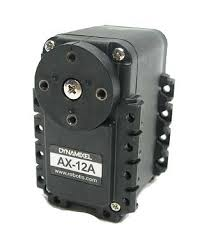
\includegraphics[width=0.3\textwidth]{dynamixel.jpg}
  \caption{An Ax-12A Dynamixel smart servo actuator.}
\label{fig:dynamixel}
\end{figure}

To supply this servo, it is recommended to use a source of 9 to 12 Volts. However, with our limited power supply it would have been needed to either switch to another power supply with higher voltage, or use a step-up voltage regulator. While testing with the arduone shield board mounted on the arduino Mega, it was observed that the smart servo didn't need that much power, and worked just fine with a power supply of 7.2 Volts. Since the board that was going to be used for the control of the dynamixel motor was not the Arduone board designed for this purpose, but the arduino micro, some modifications had to be made. Indeed, the Dynamixel actuator does not work with a full duplex serial communication protocol, but instead a half-duplex one. This means that there is only one available wire for both transmitting and receiving data. To manage to control this servo with an arduino micro, both Tx and Rx lines were connected, with a resistance of $100 \Omega$ to the Tx pin. This would prevent a short circuit from happening to the Tx pin, as the Rx pin was configured as input, and is thus protected from such a thing to happen. After this procedure, the Dynamixel worked well with 7.2 V power supply and a half duplex communication with the arduino micro.

During tests however, it was also observed that the dynamixel struggled a bit to lift the whole shovel, and since the mechanical structure of the robot was symmetric, it was possible to add a second dynamixel, connected in daisy-chain with the first one. However, the desynchronisation of the two motors, and the hyperstaticity of the assembly made them block each other, so only one motor was used. It was then not possible to lift the elevator partially.